\documentclass[pdf]{beamer}
\usepackage[utf8]{inputenc}
\usepackage{amsmath}
\usepackage{amssymb}
\usepackage{url}
\usepackage{outlines}
\usepackage{booktabs}
\usepackage[font=scriptsize,labelfont=bf,tableposition=top]{caption}
\setbeamertemplate{caption}[numbered]
\graphicspath{{media/}}

\usefonttheme{serif}
\usetheme{metropolis} 
\definecolor{srsblue}{HTML}{434e9e} 

\setbeamercolor{palette primary}{bg=srsblue,fg=white}
\setbeamercolor{palette secondary}{bg=black,fg=white}
\setbeamercolor{palette tertiary}{bg=srsblue,fg=white}
\setbeamercolor{palette quaternary}{bg=srsblue,fg=white}
\setbeamercolor{structure}{fg=srsblue}
\setbeamercolor{section in toc}{fg=srsblue}
\setbeamercolor{title separator}{fg=srsblue}
\setbeamercolor{subsection in head/foot}{bg=white,fg=white}
\beamertemplatenavigationsymbolsempty
\setbeamercolor{frametitle}{fg=white,bg=srsblue}
\setbeamertemplate{items}[circle]
\setbeamercolor{progress bar}{fg=srsblue,bg=srsblue}
\metroset{block=fill}
\setbeamertemplate{bibliography item}{}
\setbeamertemplate{bibliography entry title}{}
\setbeamertemplate{bibliography entry location}{}
\setbeamertemplate{bibliography entry note}{}

\title[Primality Testing]{Probabilistic Primality Testing and Analysis of Probabilistic AKS}
\author[Emilie Ma]{Emilie Ma}

\date[SRS'21]{Summer Research School 2021\\Apriltsi, Bulgaria}

\begin{document}

\begin{frame}
    \thispagestyle{empty}
    \titlepage
\end{frame}
\addtocounter{framenumber}{-1}

\section{Introduction}
\begin{frame}{Introduction}
    \fontsize{8}{9}\selectfont
    \begin{block}{Abstract}
        This paper aims to analyze the Fermat, the Euler (Solovay-Strassen), and the Miller-Rabin primality tests, three well-known probabilistic algorithms based on Fermat's little theorem. The Agarwal-Kayal-Saxena test, the first polynomial time deterministic primality test developed, is also discussed, as well as a proposal for a new probabilistic adaptation. This probabilistic AKS was found to deliver significant running time decreases, at the expense of eliminating determinism and passing a considerable amount of pseudoprimes.
    \end{block}
    \pause
    \normalfont
    \begin{itemize}
        \item{In layman's terms: looked at a variety of tests for checking if a number is prime, and analyzed their performance with regards to speed and accuracy}
    \end{itemize}
\end{frame}

\section{Primality Testing}
\begin{frame}{Primality Testing}
    \begin{outline}
        \1{Why is primality testing important?}
        \2{Modern cryptography and cybersecurity}
        \2{Used in verifying prime numbers}
        \2{Generates a random number, runs through primality test, if prime, then OK for use}
        \pause
        \1{Well-known primality tests include the Fermat, Euler (Solovay-Strassen), Miller-Rabin, and Agarwal-Kayal-Saxena (AKS) tests}
    \end{outline}
\end{frame}

\subsection{Probabilistic vs Deterministic}
\begin{frame}{Probabilistic vs Deterministic}
    \begin{outline}
        \1{The first three tests mentioned above (Fermat, Euler, and Solovay-Strassen) are probabilistic}
        \2{\emph{Probabilistic} $\rightarrow$ element of randomness}
        \2{\emph{Deterministic} $\rightarrow$ given the same input, always returns same output}
        \pause
        \1{Why wouldn't we always use deterministic tests?}
        \2{Often much slower, especially as we'll see with the AKS test}
        \2{High performance demands where 100\% accuracy can be sacrificed}
        \pause
        \1{Research goal: how can we take the best of both worlds of probabilistic and deterministic tests?}
    \end{outline}
\end{frame}

\section{Background Theory}
\begin{frame}{Preliminary Notes}
    \begin{outline}
        \1{Assumes a basic knowledge of modular congruences}
        \1{All $\log{n}$ shown are $\log_2{n}$ unless otherwise marked}
    \end{outline}
\end{frame}

\subsection{Fermat Primality Test}
\begin{frame}{Fermat Primality Test}
    \begin{outline}
        \1{Relies on Fermat's Little Theorem: for any integer $a$ and any prime $p$, \[a^p \equiv a \pmod{p} \leftrightarrow a^{(p - 1)} \equiv 1 \pmod{p}\]}
        \pause
        \1{Fermat's primality test chooses $k$ random integers $a$ to run this congruence on}
        \2{Passing higher $k$ values indicates a higher probability that the number is prime}
        \pause
        \1{However, certain composite numbers (like Carmichael numbers) pass Fermat's primality test}
        \2{This means there's a chance a \emph{pseudoprime} will be passed}
    \end{outline}
\end{frame}

\begin{frame}{Fermat Primality Test}
    \begin{outline}
        \1{This algorithm runs in $O(k \times \log{n})$ time complexity}
        \2{Each of the modular exponentiations takes $O(\log{n})$, and there are $k$ exponentiations}
    \end{outline}
\end{frame}

\subsection{Euler Primality Test}
\begin{frame}{Euler Primality Test}
    \begin{outline}
        \1{Utilizes on Euler's Theorem: for any integer $a$ and any prime $p$ where $a$ and $p$ are coprime, \[a^{\phi(n)} \equiv 1 \pmod{p}\]}
        \2{The $\phi(n)$ function is the totient function, which returns $p-1$ for all prime $p$}
        \2{This is a generalization of Fermat's Little Theorem}
    \end{outline}
\end{frame}

\begin{frame}{Euler Primality Test}
    \begin{outline}
        \1{Since $a^{\phi(n)} \equiv 1 \pmod{p}$, $a^{\phi(n) / 2} \equiv 1 \pmod{p}$ is
        \[
            a^{\phi(n) / 2} \equiv \begin{cases}
                \;\;\,1\pmod{n}& \text{ when $x$ s.t. } a\equiv x^2 \pmod{n}\\
                -1\pmod{n}& \text{ when no such integer.}
            \end{cases}
        \]}
        \pause
        \1{This forms the criteria for the Legendre symbol $\left(\frac{a}{p}\right)$, which is only defined for odd primes $p$}
        \2{To allow the Euler primality test to be computed for nonprimes, the Jacobi symbol generalization is used}
        \pause
        \1{As with the Fermat test, $k$ random bases $a$ are tested}
        \2{More accurate than Fermat, but there remains a chance a pseudoprime is passed}
        \pause
        \1{The Euler test runs in $O(k \times \log^3{n})$ time complexity}
        \2{Each of the coprime to $n$, Jacobi symbol, and modular exponentiations checks takes $O(\log{n})$, so $\log{n}$ has a power of 3, and there are $k$ bases to check}
    \end{outline}
\end{frame}

\subsection{Miller-Rabin Primality Test}
\begin{frame}{Miller-Rabin Primality Test}
    \begin{outline}
        \1{The Miller-Rabin Primality test uses different congruences instead, checking for:
        \begin{gather*}
            a^d \equiv 1 \pmod{n} \\
            a^{(2^r \times d)} \equiv -1 \text{ for some $r$ such that $0 \leq r < s$}
        \end{gather*}
        where $n$ is rewritten as $2^s \times d + 1$ and $0 \le a \le n$.}
        \2{$n-1 = 2^s \times d$, so if $a^d \equiv \pm 1 \pmod{n}$, $n$ is a \emph{strong probable prime}}
        \2{Strong probable $\leftrightarrow$ Miller-Rabin verified}
        \pause
        \1{This test passes far fewer pseudoprimes than Fermat or Euler tests}
        \2{Between $10^5$ and $10^6$, 167 Fermat, 78 Euler, and 30 strong pseudoprimes found \cite{pomerance_pseudoprimes_1980}}
        \pause
        \1{The Miller-Rabin test also runs in $O(k \times \log^3{n})$ time complexity}
    \end{outline}
\end{frame}

\subsection{Agarwal-Kayal-Saxena Primality Test}
\begin{frame}{Agarwal-Kayal-Saxena Primality Test}
    \begin{outline}
        \1{Notable for being the first deterministic primality that runs in polynomial time (bounds of $\widetilde{O}(\log^{15/2}{n})$)}
        \pause
        \1{Based on the theorem that for any $a$ where $a$ is coprime to $n$ and where $n \geq 2$, the following holds within the polynomial ring $\mathbb{Z}[x]$:
        \[
            (X + a)^n \equiv X^n + a \pmod{n}
        \]}
    \end{outline}
\end{frame}

\begin{frame}{Agarwal-Kayal-Saxena Primality Test}
    \begin{outline}
        \1{The test has 5 key steps:}
        \begin{itemize}
                \pause
            \item{Ensure $n$ is not a perfect power ($n = a^k$); if it is, $n$ is composite}
                \pause
            \item{Find smallest $r$ such that $\textrm{ord}_r(n) \ge \log{n}^2$}
                \pause
            \item{Check that no number $a$ $2 \leq a \leq r$ divides $n$; if $a$ does, $n$ is composite}
                \pause
            \item{Check $n \leq r$; if so, $n$ is prime.}
                \pause
            \item{Compute all $(X + a)^n \equiv X^n + a \pmod{n}$ for $1 \leq a \leq \lfloor \sqrt{\phi(r)} \log{n} \rfloor$; if $n$ passes all these tests, it is prime, otherwise it is composite.}
        \end{itemize}
    \end{outline}
\end{frame}

\subsection{Probabilistic AKS Primality Test}
\begin{frame}{Probabilistic AKS Primality Test}
    \begin{outline}
        \1{Step 5 in the AKS algorithm has very high bounds, and is very expensive computationally to check - how can we change these bounds to make AKS faster?}
        \pause
        \1{Probabilistic AKS: this research project's proposal for a new variant of AKS}
        \2{Instead of checking all $a$ $1 \leq a \leq \lfloor \sqrt{\phi(r)} \log{n} \rfloor$, choose $k$ random $a$ values from that range to check}
        \2{Similar idea as the random choice of $a$ in the Fermat, Euler, and Miller-Rabin tests}
    \end{outline}
\end{frame}

\begin{frame}{Probabilistic AKS Primality Test}
    \begin{outline}
        \1{Removing the determinism, but reducing the runtime}
        \pause
        \2{Step 5 dominates the time taken, due to high numbers of computations depending on the value of $r$, bounded at $O(\log^3{n})$ \cite{agrawal_primes_2004}}
        \pause
        \2{Each of the $(X + a)^n \equiv X^n + a \pmod{n}$ equations requires $O(r \times \log^2{n})$ computations}
        \pause
        \2{Instead of having to check $\lfloor \sqrt{\phi(r)} \log{n} \rfloor$ calculations ($O(\sqrt{(\log^3{n})} \times \log{n}) = O(\log^{5/2}{n})$), $k$ equations can be checked, leading to a worst-case complexity of:
        \[
            \widetilde{O}(k \times r \times \log^2{n}) = \widetilde{O}(k \times \log^5{n})
        \]}
        \pause
        \2{With $r$'s lower bound proven as $2 + \log^2{n}$ \cite{terzian_aks_2013}, this could be as low as $\widetilde{O}(k \times \log^4{n})$}
    \end{outline}
\end{frame}

\section{Analysis Methods}
\begin{frame}{Analysis Methods}
    \begin{outline}
        \1{To consistently analyze the four primality tests (AKS was not tested for pseudoprimes as it is proven correct and would have taken too long), integers in the range $10^5 \leq x \leq 10^6$ were randomly chosen}
        \2{For the Fermat, Euler, and Miller-Rabin tests, $10^4$ integers were chosen}
        \2{For probabilistic AKS, $10^2$ integers were chosen (as testing $10^4$ integers over a large number of trials was infeasible time-wise for this analysis)}
        \pause
        \1{Ran the primality test with a variety of $k$ values}
    \end{outline}
\end{frame}

\begin{frame}{Analysis Methods}
    \begin{outline}
        \1{Sympy's \texttt{isprime} function was used as a reference to test for primality}
        \2{The numbers marked as prime by the primality test being analyzed were compared with the \texttt{isprime} results}
        \pause
        \1{The 'optimal' $k$ values (those that passed the lowest number of pseudoprimes) were recorded, as well as running time elapsed, minimum and maximum number of pseudoprimes passed, and other relevant variables}
        \pause
        \1{All the data collected can be found at \href{https://github.com/kewbish/srs/tree/master/dataset}{kewbish/srs} on GitHub}
    \end{outline}
\end{frame}

\section{Results}
\begin{frame}{Average pseudoprimes vs. $k$ base trials}
    \begin{columns}[t, onlytextwidth]
        \begin{column}{0.65\textwidth}
            \begin{figure}[h!]
                \caption{The effect of increasing the number of base trials $k$ on pseudoprimes passed}
                \label{fig:pprimes_v_bases}
                \centering
                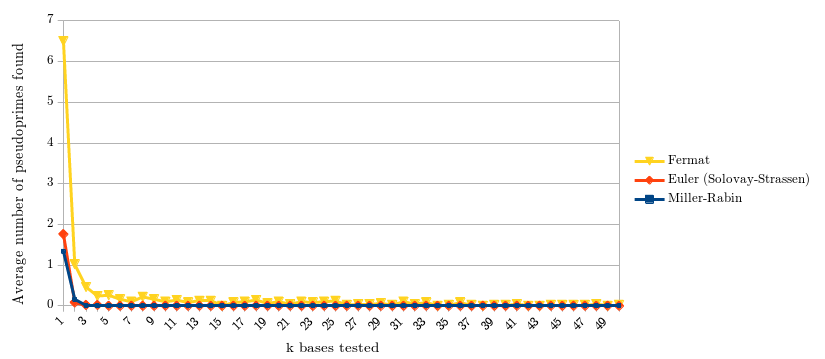
\includegraphics[width=\textwidth]{pprimes_v_bases}
            \end{figure}
        \end{column}
        \begin{column}{0.35\textwidth}
            \fontsize{8}{9}\selectfont
            \begin{outline}
                \1{All tests pass larger numbers of pseudoprimes with higher $k$ values, expected due to probability}
                \pause
                \1{At $k=1$, Fermat passed the most pseudoprimes (6.5), Euler passed 3.2, Miller-Rabin 3.3}
                \pause
                \1{Miller-Rabin begins to pass low (<0.1) pseudoprimes first}
                \pause
                \1{Both Euler and Miller-Rabin consistently pass 0 pseudoprimes at higher $k$ values}
            \end{outline}
        \end{column}
    \end{columns}
\end{frame}

\begin{frame}{Average pseudoprimes vs. trial number}
    \begin{columns}[t, onlytextwidth]
        \begin{column}{0.65\textwidth}
            \begin{figure}[h!]
                \caption{Average pseudoprimes passed across all $1 \leq k \leq 50$ values per trial}
                \label{fig:pprimes_v_trial}
                \centering
                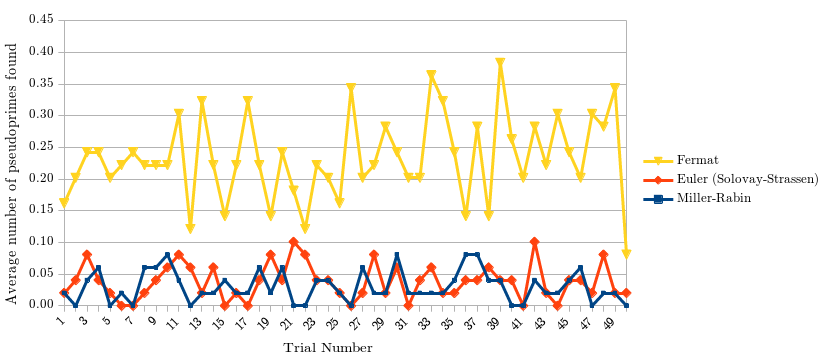
\includegraphics[width=\textwidth]{pprimes_v_trial}
            \end{figure}
        \end{column}
        \begin{column}{0.35\textwidth}
            \fontsize{8}{9}\selectfont
            \begin{outline}
                \1{Fermat has a higher average at around 0.2327 pseudoprimes, whereas Euler and Miller-Rabin pass 0.0380 and 0.0303 pseudoprimes respectively}
                \pause
                \1{Miller-Rabin has the smallest range of numbers of pseudoprimes passed}
            \end{outline}
        \end{column}
    \end{columns}
\end{frame}

\begin{frame}{Probabilistic primality tests - accuracy}
    \begin{columns}[t, onlytextwidth]
        \begin{column}{0.48\textwidth}
            \begin{figure}
                \setcounter{figure}{0}
                \caption{The effect of increasing the number of base trials $k$ on pseudoprimes passed}
                \centering
                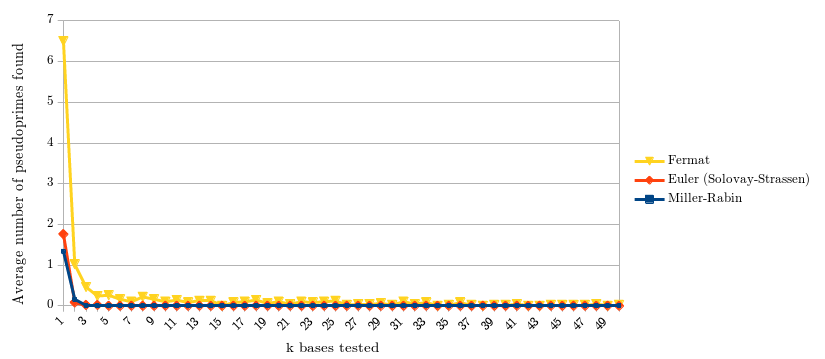
\includegraphics[width=\textwidth]{pprimes_v_bases}
            \end{figure}
        \end{column}
        \begin{column}{0.48\textwidth}
            \begin{figure}
                \setcounter{figure}{1}
                \caption{Average pseudoprimes passed across all $1 \leq k \leq 50$ values per trial}
                \centering
                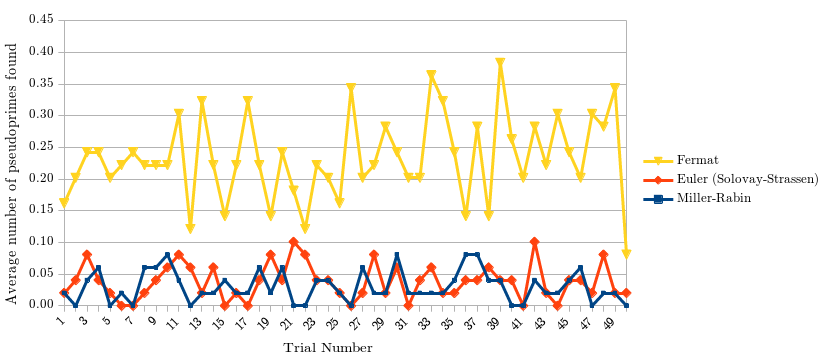
\includegraphics[width=\textwidth]{pprimes_v_trial}
            \end{figure}
        \end{column}
    \end{columns}
    \begin{outline}
        \1{Fermat consistently passed more pseudoprimes}
        \pause
        \1{Euler and Miller-Rabin appear to perform quite similarly but on average Euler will pass more pseudoprimes}
        \pause
        \1{Supported by the results of Pomerance, Selfridge, and Wagstaff, as well as by Monier's findings \cite{pomerance_pseudoprimes_1980}\cite{monier_evaluation_1980}}
    \end{outline}
\end{frame}

\begin{frame}{Running time vs. $k$ base trials}
    \begin{columns}[t, onlytextwidth]
        \begin{column}{0.65\textwidth}
            \begin{figure}[h!]
                \caption{The effect of increasing the number of base trials $k$ on running time elapsed}
                \label{fig:time_v_bases}
                \centering
                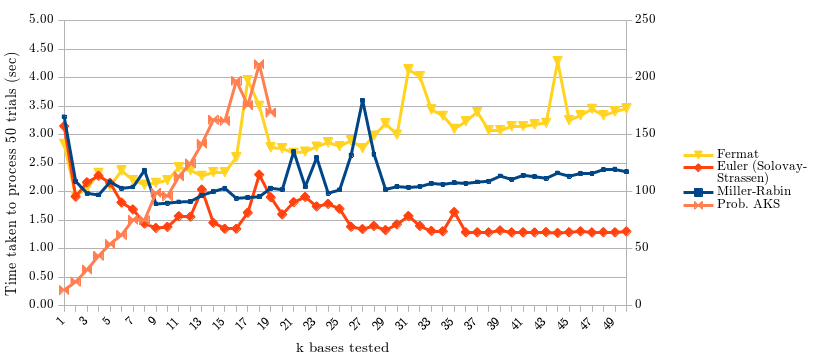
\includegraphics[width=\textwidth]{time_v_bases}
            \end{figure}
        \end{column}
        \begin{column}{0.35\textwidth}
            \fontsize{8}{9}\selectfont
            \begin{outline}
                \1{Fermat's running time increases the most out of the existing tests, and takes the longest at any given $k$}
                \pause
                \1{Euler has a downwards slope of around -0.01sec/$k$, and is even faster than Miller-Rabin}
                \pause
                \1{Contrasts theoretical runtime where the expectations were Fermat < Euler = Miller-Rabin}
            \end{outline}
        \end{column}
    \end{columns}
\end{frame}

\begin{frame}{Running time vs. trial number}
    \begin{columns}[t, onlytextwidth]
        \begin{column}{0.65\textwidth}
            \begin{figure}[h!]
                \caption{Running time elapsed across all $1 \leq k \leq 100$ values per trial}
                \label{fig:time_v_trial}
                \centering
                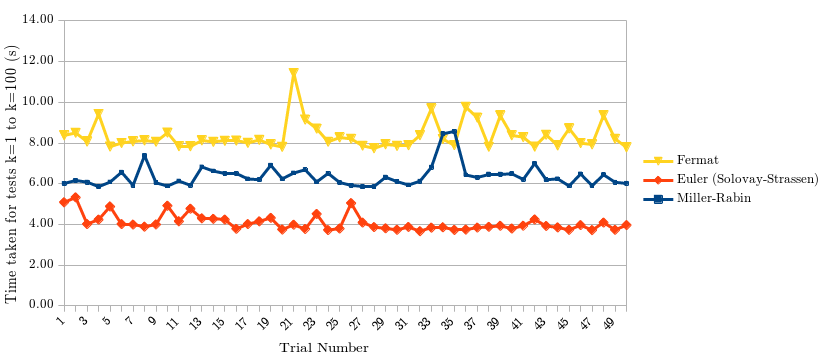
\includegraphics[width=\textwidth]{time_v_trial}
            \end{figure}
        \end{column}
        \begin{column}{0.35\textwidth}
            \fontsize{8}{9}\selectfont
            \begin{outline}
                \1{Again, contrasts expectations, with Euler outperforming Miller-Rabin, which was in turn faster than Fermat}
            \end{outline}
        \end{column}
    \end{columns}
\end{frame}

\begin{frame}{Probabilistic primality tests - runtime}
    \begin{columns}[t, onlytextwidth]
        \begin{column}{0.48\textwidth}
            \begin{figure}
                \setcounter{figure}{2}
                \caption{The effect of increasing the number of base trials $k$ on pseudoprimes passed}
                \centering
                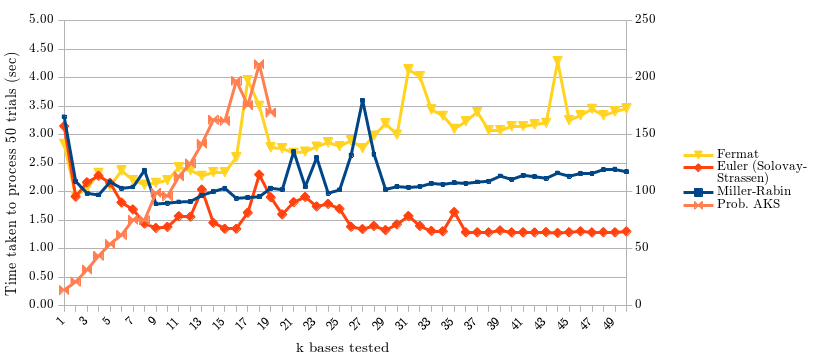
\includegraphics[width=\textwidth]{time_v_bases}
            \end{figure}
        \end{column}
        \begin{column}{0.48\textwidth}
            \begin{figure}
                \setcounter{figure}{3}
                \caption{Average pseudoprimes passed across all $1 \leq k \leq 50$ values per trial}
                \centering
                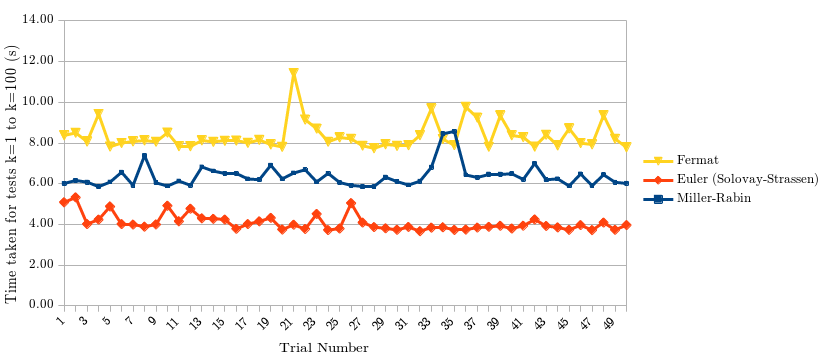
\includegraphics[width=\textwidth]{time_v_trial}
            \end{figure}
        \end{column}
    \end{columns}
    \begin{outline}
        \1{A possible explanation for more efficient runtime of Euler and Miller-Rabin is the speed at which numbers are discarded as composite}
        \2{The congruences used in the Euler and Miller-Rabin tests may do so more quickly - though this has not been theoretically verified yet}
    \end{outline}
\end{frame}

\begin{frame}{Projected pseudoprimes vs. $k$ value}
    \begin{columns}[t, onlytextwidth]
        \begin{column}{0.65\textwidth}
            \begin{figure}[h!]
                \caption{Projected average number of pseudoprimes passed by probabilistic AKS versus other tests}
                \label{fig:paks_proj_pprimes_v_bases}
                \centering
                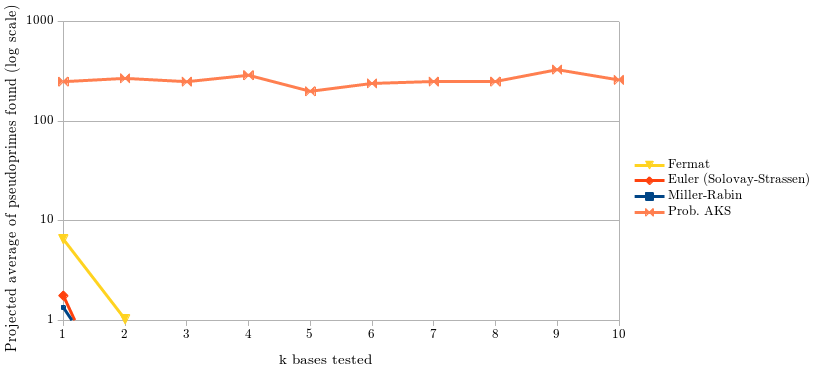
\includegraphics[width=\textwidth]{paks_proj_pprimes_v_bases}
            \end{figure}
        \end{column}
        \begin{column}{0.35\textwidth}
            \fontsize{8}{9}\selectfont
            \begin{outline}
                \setbeamerfont{itemize/enumerate subbody}{size=\scriptsize}
                \1{Significant increase in number of projected pseudoprimes passed by probabilistic AKS compared to the existing tests (~200 vs. <10)}
                \2{Projection method: multiply pseudoprimes found by $10^2$}
                \pause
                \1{Due to the relatively very low $k$ values tested for probabilistic AKS}
            \end{outline}
        \end{column}
    \end{columns}
\end{frame}

\begin{frame}{$k$ value trials for probabilistic AKS}
    \begin{table}
        \caption{Number of pseudoprimes passed at given $k$ values\label{table:paks_pprimes_v_bases}}
        \begin{tabular}{l|lllllll|l}
            \toprule
            k-value & \multicolumn{7}{l|}{Pseudoprimes passed} & Average pseudoprimes  \\
            & 0 & 1 & 2 & 3 & 4 & 5 & 6                &                       \\
            \hline
            100     & 0 & 1 & 2 & 1 & 3 & 0 & 2                & 3.4                   \\
            200     & 1 & 0 & 4 & 0 & 3 & 0 & 0                & 2.6                   \\
            300     & 3 & 0 & 4 & 1 & 1 & 0 & 0                & 1.7                   \\
            400     & 4 & 0 & 4 & 2 & 0 & 0 & 0                & 1.4                   \\
            \bottomrule
        \end{tabular}
    \end{table}
    \begin{outline}
        \1{Downward trends for pseudoprimes passed also observed for probabilistic AKS}
        \2{The $k$ values required to pass low pseudoprimes are significantly higher than that of the existing probabilistic tests due to the nature of the deterministic AKS algorithm}
    \end{outline}
\end{frame}

\begin{frame}{Running time of probabilistic AKS}
    \begin{columns}[t, onlytextwidth]
        \begin{column}{0.48\textwidth}
            \begin{figure}
                \setcounter{figure}{2}
                \caption{The effect of increasing the number of base trials $k$ on pseudoprimes passed}
                \centering
                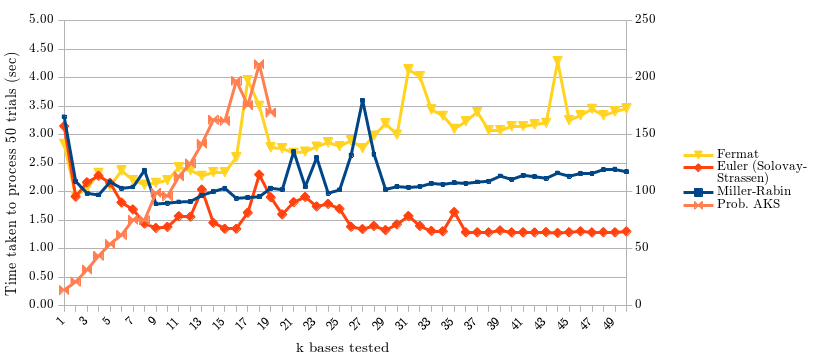
\includegraphics[width=\textwidth]{time_v_bases}
            \end{figure}
        \end{column}
        \begin{column}{0.48\textwidth}
            \begin{figure}
                \setcounter{figure}{6}
                \caption{Elapsed running time for probabilistic versus deterministic AKS}
                \centering
                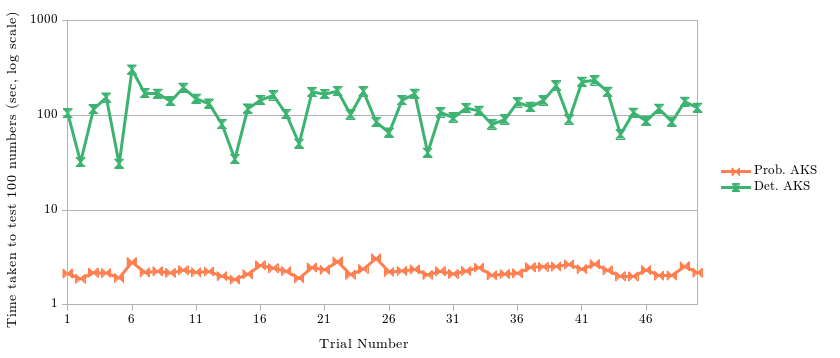
\includegraphics[width=\textwidth]{paks_v_daks}
            \end{figure}
        \end{column}
    \end{columns}
    \begin{outline}
        \setbeamerfont{itemize/enumerate body}{size=\small}
        \1{Probabilistic AKS is considerably slower than the existing primality tests, but also significantly faster than deterministic AKS}
        \2{Discrepancies in runtime from probabilistic AKS and existing primality tests can be attributed to time complexity}
    \end{outline}
\end{frame}

\begin{frame}{All pseudoprimes passed $10^5 \leq x \leq 10^6$}
    \begin{columns}[t, onlytextwidth]
        \begin{column}{0.65\textwidth}
            \begin{figure}[h!]
                \caption{Distribution of pseudoprimes found between $10^5$ and $10^6$ for probabilistic primality tests}
                \label{fig:pprimes_passed}
                \centering
                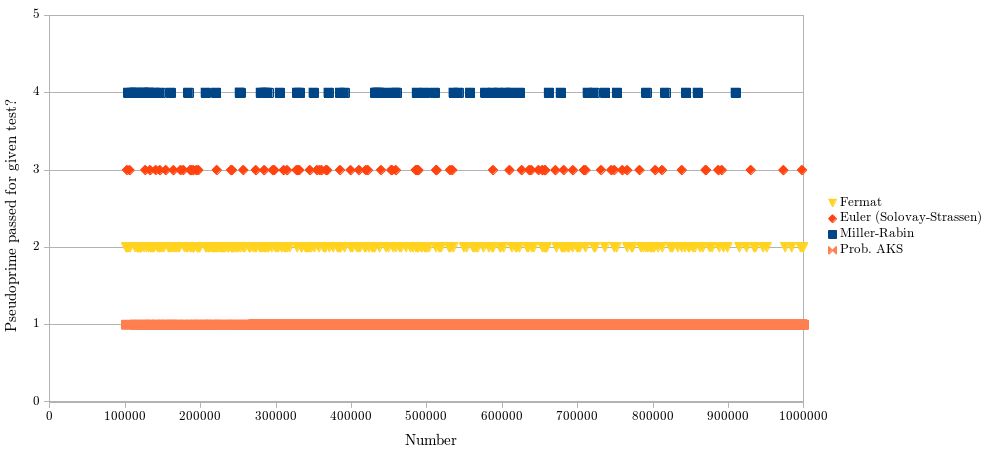
\includegraphics[width=\textwidth]{pprimes_passed}
            \end{figure}
        \end{column}
        \begin{column}{0.35\textwidth}
            \fontsize{8}{9}\selectfont
            \begin{outline}
                \setbeamerfont{itemize/enumerate subbody}{size=\scriptsize}
                \1{AKS passes by far the greatest pseudoprimes (11524), followed by Fermat (274), Euler (81), and Miller-Rabin (63)}
                \2{Contrasts with Pomerance et. al's findings, but may be attributed to base analysis differences \cite{pomerance_pseudoprimes_1980}}
            \end{outline}
        \end{column}
    \end{columns}
\end{frame}

\subsection{Sources of Error}
\begin{frame}{Sources of Error}
    \begin{outline}
        \1{Several possible sources of error were identified in this research project}
        \pause
        \2{Insufficient bounds of numbers tested; higher amounts of pseudoprimes are found with larger numbers}
        \pause
        \2{Inconsistent amount of numbers tested for each primality trial: the fifty trials of $10^4$ with the Fermat, Euler, and Miller-Rabin tests versus the twenty of $10^2$ for probabilistic AKS}
        \pause
        \2{Potentially misleading \texttt{isprime} Sympy function used; also relies on probabilistic methods}
    \end{outline}
\end{frame}

\subsection{Future Research}
\begin{frame}{Future Research}
    \begin{outline}
        \1{To address the sources of error discussed earlier, future research to be conducted includes:}
        \pause
        \2{Experimenting with larger bounds for each primality test; perhaps $10^7$ to $10^9$}
        \pause
        \2{Running additional trials with the full $10^4$ numbers for probabilistic AKS, and increasing the number of trials run for the other primality tests as well}
        \pause
        \2{Precomputing an array of deterministically verified (with AKS) values to check primality against}
        \pause
        \2{Adjusting the bounds of $r$ in probabilistic AKS to further improve the theoretical runtime complexity}
    \end{outline}
\end{frame}

\section{Conclusion}
\begin{frame}{Conclusion}
    \begin{outline}
        \1{Fermat: low efficiency, and low accuracy $\rightarrow$ simple to implement, but not practical}
        \pause
        \1{Euler: high efficiency, and decent accuracy $\rightarrow$ best in speed-driven scenarios}
        \pause
        \1{Miller-Rabin: relatively high efficiency, and higher accuracy than Euler $\rightarrow$ recommended when practical accuracy is key}
        \pause
        \1{Deterministic AKS: no pseudoprimes passed, and very slow to run $\rightarrow$ good for applications where speed is irrelevant}
        \pause
        \1{Probabilistic AKS: high numbers of pseudoprimes passed at low $k$, much faster than deterministic AKS $\rightarrow$ may provide a suitable alternative to deterministic AKS for more practical applications given high enough $k$ values}
    \end{outline}
\end{frame}

\subsection{Future Research}
\begin{frame}{Future Research}
    \begin{outline}
        \1{To address the sources of error discussed earlier, future research to be conducted includes:}
        \pause
        \2{Experimenting with larger bounds for each primality test; perhaps $10^7$ to $10^9$}
        \pause
        \2{Running additional trials with the full $10^4$ numbers for probabilistic AKS, and increasing the number of trials run for the other primality tests as well}
        \pause
        \2{Precomputing an array of deterministically verified (with AKS) values to check primality against}
        \pause
        \2{Adjusting the bounds of $r$ in probabilistic AKS to further improve the theoretical runtime complexity}
    \end{outline}
\end{frame}


\subsection{Acknowledgements}
\begin{frame}{Acknowledgements}
    \begin{outline}
        \1{Many thanks to my mentor, Ms. Pressiana Marinova, for her unfailing guidance and support throughout SRS and the research process, her deep knowledge and clear explanations of new topics, and for always being there to answer all my questions.}
        \pause
        \1{Much gratitude also to the Summer Research School and High School Student Institute of Mathematics and Informatics for making this research inquiry experience possible, and for hosting such an organized, fun summer program.}
    \end{outline}
\end{frame}


\subsection{References}
\begin{frame}[allowframebreaks]{References}
    \nocite{*}
    \bibliographystyle{plain}
    \bibliography{references}
\end{frame}

\end{document}

